\documentclass[letterpaper, 10 pt, conference]{ieeeconf}

\IEEEoverridecommandlockouts
\overrideIEEEmargins

% Core
\usepackage{cite}
\usepackage{amsmath,amssymb,amsfonts}
\usepackage{graphicx}
\graphicspath{{Figures/}}
\usepackage{booktabs}
\usepackage{makecell}
\renewcommand\theadfont{\normalsize\bfseries}
\usepackage{array}
\usepackage{multirow}
\usepackage{siunitx}
\usepackage{bm}
\usepackage{url}
\usepackage{hyperref}
\usepackage{xcolor}
\usepackage{algorithm}
\usepackage{algorithmic}

% Floats & subfigures
\usepackage{subcaption}
\usepackage{dblfloatfix}
\usepackage{tikz}
\usetikzlibrary{arrows.meta, positioning, fit, backgrounds, calc}

\newcommand{\TODO}[1]{\textcolor{red}{\textbf{TODO:} #1}}

\title{\LARGE \bf Clearing Dense Log Piles with Imitation-Bootstrapped Reinforcement Learning}

\author{
Anonymous Authors
}
\begin{document}
\maketitle
\thispagestyle{empty}
\pagestyle{empty}

\begin{abstract}
Clearing a dense pile of logs by sequential grasping is a contact-rich manipulation problem. The scene contains hundreds of rigid bodies in frictional contact, each grasp reshapes the pile, and effective strategies span long horizons.
We study this problem in simulation for a forestry log loader that must clear piles of 200 logs directly from depth-derived point clouds.
Our framework first trains a PointNet-based policy via behavior cloning (BC) on demonstrations from a privileged-state heuristic, then fine-tunes with reinforcement learning (RL) via Proximal Policy Optimization (PPO) using an asymmetric actor-critic.
The resulting policy maintains expert-level clearing ($98.2$\%) while producing $15$\% more stable grasps than BC, from depth-derived point clouds alone.
From-scratch RL plateaus well below full clearing despite observation and reward ablations, while RL fine-tuning over a BC-initialized policy improves per-grasp quality beyond what the demonstrator achieves.
\end{abstract}

\begin{keywords}
robot learning, multi-object grasping from dense clutter, behavior cloning, reinforcement learning fine-tuning, contact-rich simulation
\end{keywords}

\section{INTRODUCTION}
The forestry industry is increasingly looking for autonomous solutions for heavy machinery used in mills and forests to improve safety and productivity~\cite{lindroos2017forestry}.
One key subtask carried out by log-loading machines is log-pile clearing: repeatedly grasping multiple logs from a rack or pile and removing them.
This setting is challenging because (i) the scene is densely cluttered with hundreds of rigid-body logs in frictional contact, (ii) each grasp disturbs the pile through contact cascades, continuously reshaping the configuration for subsequent attempts, and (iii) no two pile configurations are alike, so a targeting strategy must be robust to diverse arrangements.

\begin{figure}[b]
\centering
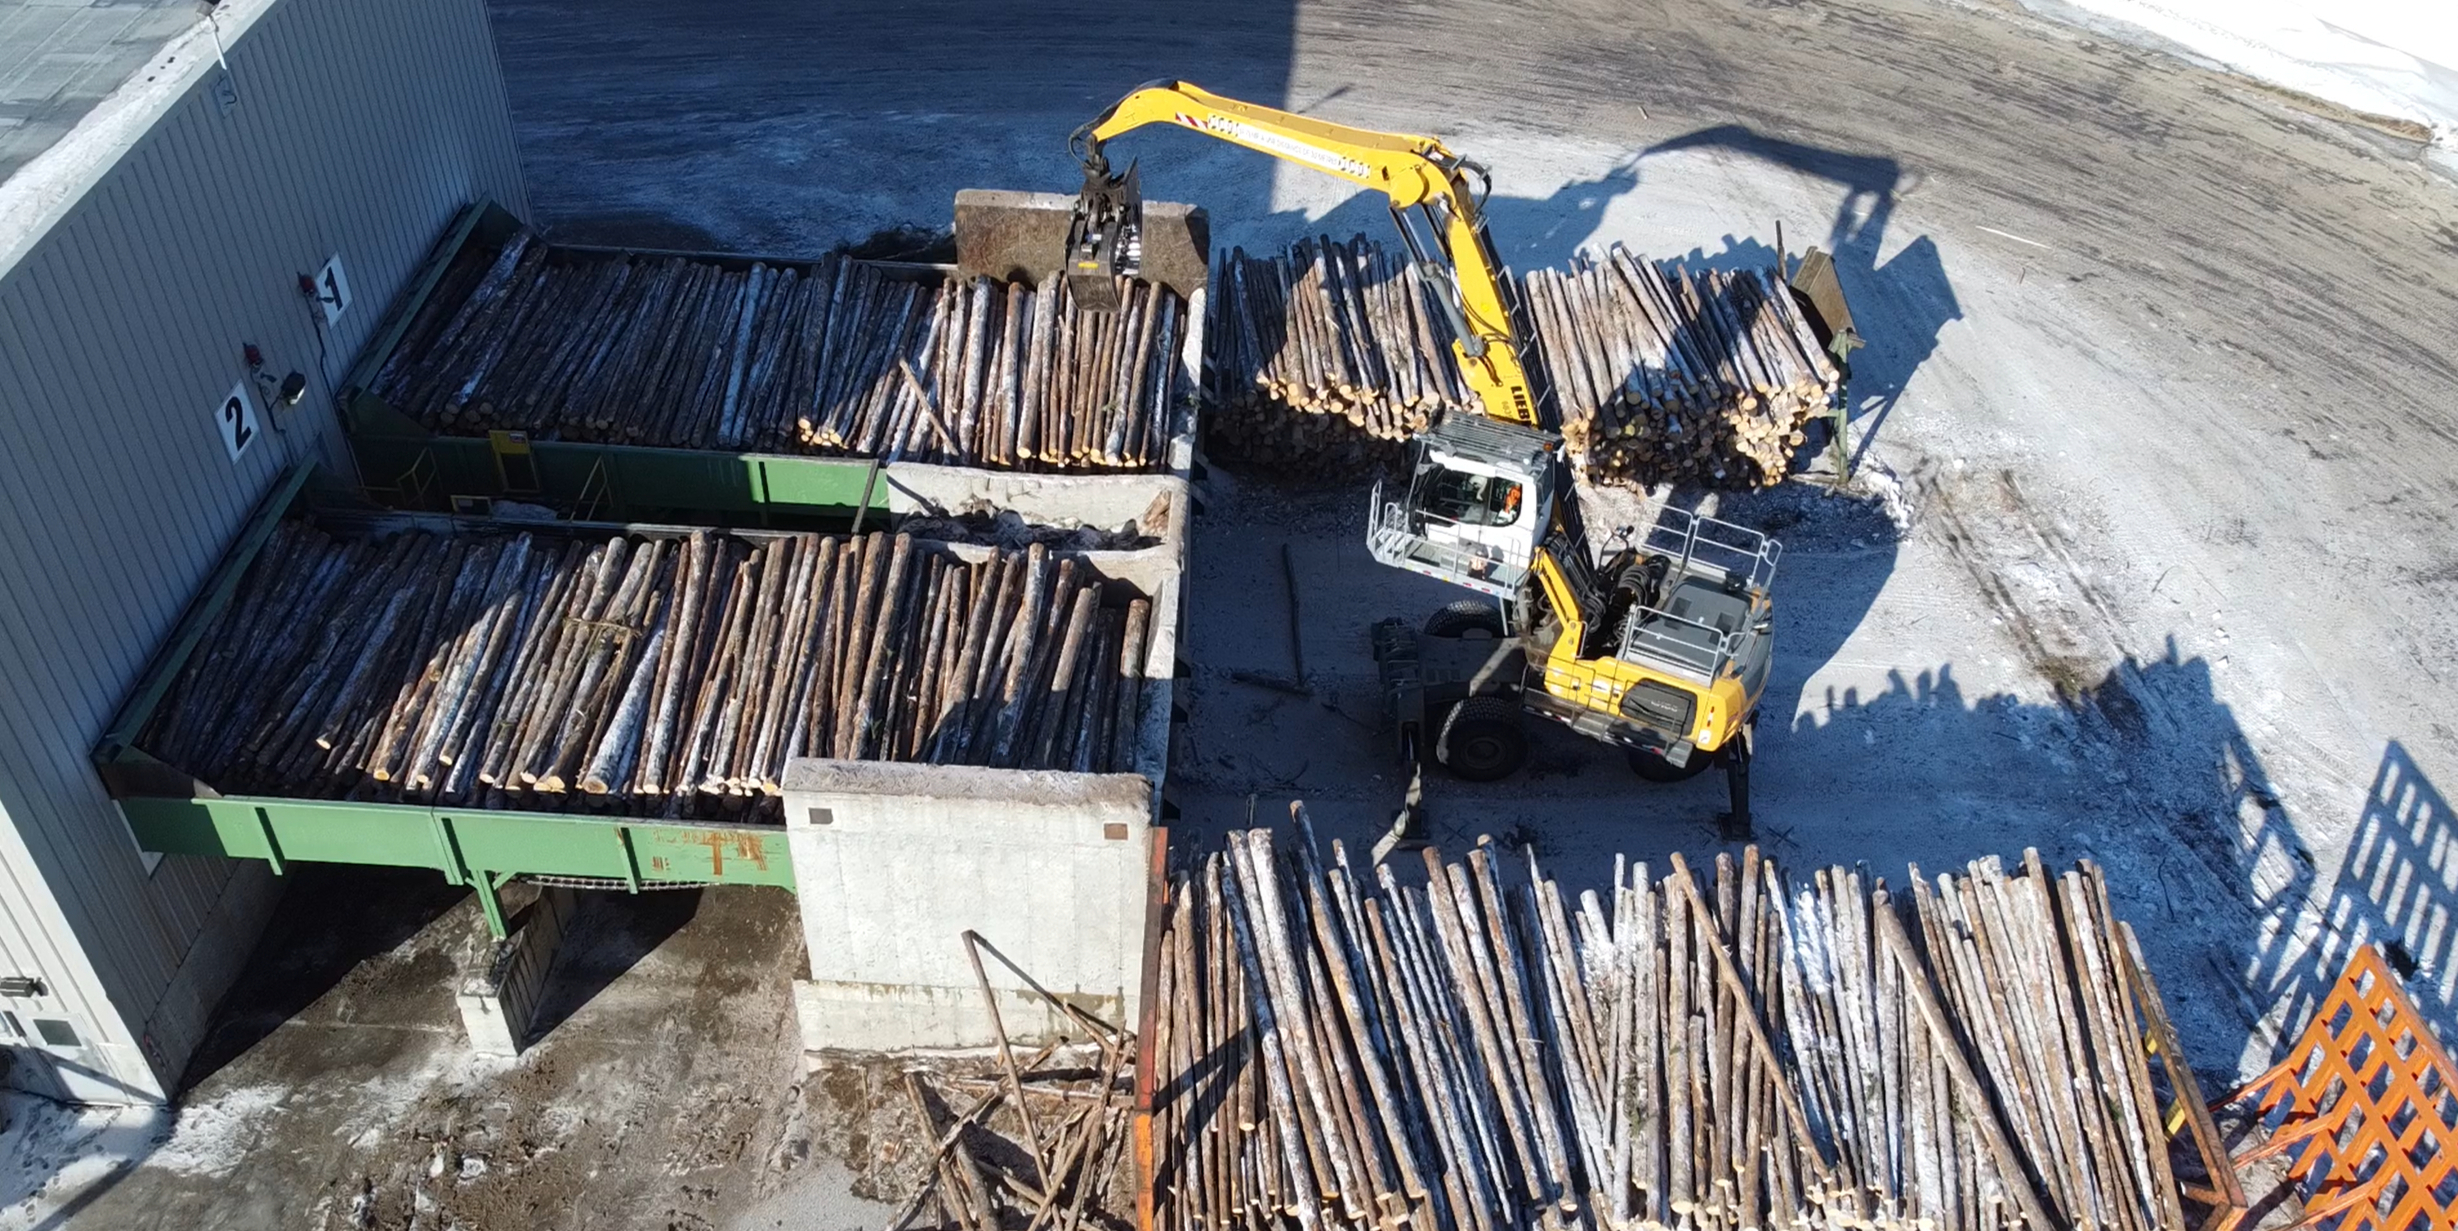
\includegraphics[width=\columnwidth]{mill.jpg}
\caption{A log loader clearing piles at a millyard infeed deck.}
\label{fig:mill}
\end{figure}

We address the grasp target selection problem: given a raw point cloud derived from a stereo depth camera, where should the crane place and orient the grapple to clear the pile efficiently?
We deliberately separate this high-level targeting decision from low-level motion execution.
Concretely, we implement a grasp-and-remove simulator in Isaac Lab~\cite{mittal2025isaaclab} where each environment step is one complete pick attempt: a policy selects where to grasp, a fixed finite-state machine (FSM) handles execution, and grasped logs are removed rather than deposited, allowing us to measure clearing progress without modeling the log placement dynamics.

Existing work on autonomous log grasping addresses small-scale settings: single-log pick-and-place, small groupings of two to seven logs, or grasp prediction without sequential clearing.
We scale to full pile-level clearing with dense frictional contact dynamics among hundreds of logs.
To our knowledge, this is the first study of learned sequential grasp targeting at this pile scale.
Dense log-pile clearing poses a difficult exploration problem for RL: reward signal is sparse across long episodes of sequential grasps, and the high-dimensional point-cloud observation space compounds the challenge.
Our approach is to first train a policy via BC on demonstrations from a privileged-state heuristic, then fine-tune with RL.
The demonstration data spans the complete clearing trajectory, giving the RL agent the distributional coverage it struggles to acquire through exploration alone.

Our main contributions are:
\begin{itemize}
    \item A grasp-and-remove task formulation for sequential dense log-pile clearing (200 logs, 30-grasp horizons) and a behavior cloning to reinforcement learning (BC$\to$RL) pipeline that learns to clear dense piles via stable sequential grasps from raw point clouds.
    \item A four-method comparison (heuristic, RL, BC, BC$\to$RL) showing that from-scratch RL plateaus well below full clearing despite observation and reward ablations, while BC from raw point clouds matches the privileged-state heuristic and BC$\to$RL fine-tuning improves per-grasp stability beyond both BC and the heuristic while maintaining near-complete clearing.
\end{itemize}

\section{RELATED WORK}

\subsection{Grasping in Clutter}
Learning-based grasp detection has progressed from single isolated objects to cluttered, multi-object scenes.                                       
Deep grasp prediction networks predict grasp pose directly from depth images~\cite{morrison2018closing, kumra2017robotic}, and large-scale
synthetic datasets have enabled robust grasp planning without real-world
training data~\cite{mahler2017dexnet}.
Sequential decluttering has been studied in bin picking, where learned
policies account for how each pick changes the
heap~\cite{mahler2017sequential} and pushing is combined with grasping to
handle dense clutter~\cite{zeng2018learning}.
Applications extend to natural-resource handling such as forestry log loading~\cite{wallin2024multilog}.

However, these works typically involve heterogeneous objects of varied shape and size in loose arrangements, where clutter arises from random placement rather than dense packing.
Our setting differs in important ways: we perform power grasps from dense piles of cylindrical logs of uniform geometry that are initially stacked in ordered layers.
The homogeneity and tight packing mean that logs are in extensive frictional contact with their neighbors, and each grasp attempt (which captures multiple logs simultaneously) disturbs the pile, causing settling, rolling, and potential knock-offs that reshape the configuration for all subsequent attempts.

\subsection{Learning for Log Grasping and Forestry Crane Control}
A growing body of work applies learning methods to log grasping and forestry crane automation, though existing approaches address smaller-scale settings than the one considered here.

For grasp prediction, Wallin et~al.~\cite{wallin2024multilog} use RL with virtual visual servoing for multi-log grasping from small groupings of two to five logs in simulation, separating image segmentation from Cartesian crane control; the pile dynamics are limited to a handful of objects.
F{\"a}lldin et~al.~\cite{falldin2025synthesizing} train a U-Net CNN on synthetic RGB-D images to predict grasp poses for small clusters of up to seven logs, with an open-loop kinematic controller; their work focuses on grasp prediction from synthetic data and does not address sequential clearing or pile-scale dynamics.
Ayoub et~al.~\cite{ayoub2023grasp} propose a CNN-based grasp planner for a log-loading forestry machine that predicts a grasp configuration from a depth image for small log clusters, validated in simulation and on a real log loader.

For crane control, Vu et~al.~\cite{vu2025autonomous} present a MuJoCo-based forestry crane simulator and benchmark RL velocity controllers for grasping single logs of varying diameter (simulation only).
Kurinov et~al.~\cite{kurinov2025reinforcement} train an RL agent for the full single-log pick-and-place pipeline (locate, grasp, transport, load) in Isaac Gym simulation, but with one log at a time.
Jebellat et~al.~\cite{jebellat2025designing} use dynamic programming to design anti-sway trajectories for a log loader end effector.
These works address individual subtasks but none tackle sequential dense-pile clearing at the scale we consider.

More broadly, using demonstrations to initialize RL policies has been shown to overcome exploration challenges in contact-rich manipulation~\cite{rajeswaran2018learning, nair2018overcoming}, and asymmetric actor-critic architectures (where the critic receives privileged state information unavailable to the actor) have proven effective for learning from high-dimensional visual observations~\cite{pinto2018asymmetric}.
\section{PROBLEM FORMULATION}
\subsection{Grasp-and-Remove Task}
\label{sec:formulation}
Each environment step corresponds to a complete grasp attempt: a policy selects a grasp target, the FSM executes the approach, close, and lift, and grasped logs are removed from the scene.
This formulation is shared by all methods (heuristic, BC, RL, and BC+RL).
The state $s_t \in \mathcal{S}$ is the current pile configuration (observed via point cloud or privileged poses; Section~\ref{sec:obs}).
A grasp target is defined by the tuple
\begin{equation}
    \mathbf{g} = (x,\, y,\, z,\, \psi),
\end{equation}
where $(x, y, z)$ is the grapple position in the crane base frame and $\psi$ is the grapple yaw angle about the vertical axis.
Because the grapple is symmetric about its yaw axis, the policy represents $\psi$ via the $\pi$-periodic encoding $(\cos 2\psi, \sin 2\psi)$~\cite{morrison2018closing}, giving a 5D action $a_t \in \mathcal{A} \subset \mathbb{R}^5$ (Section~\ref{sec:actions}).
The transition $T(s_{t+1}|s_t, a_t)$ is determined by the physics simulation and FSM execution.
After each grasp attempt, an outcome evaluation measures the number of logs grasped, grapple--log alignment, and grapple stability (Section~\ref{sec:outcome}).
For RL training, this outcome is used as a scalar reward $r_t = R(s_t, a_t)$, and the full structure is treated as an episodic Markov decision process $(\mathcal{S}, \mathcal{A}, T, R, \gamma)$ with discount factor $\gamma$, where a policy $\pi$ maximizes the expected discounted return over a horizon of $H$ grasp attempts:
\begin{equation}
    \max_\pi \; \mathbb{E}_\pi \!\left[\sum_{t=0}^{H-1} \gamma^t \, r_t \right].
\end{equation}
An episode terminates when no logs remain on the rack or after a fixed horizon of $H=30$ grasp attempts.
A log leaves the rack either by being grasped and removed or by being knocked outside the workspace bounds (Section~\ref{sec:outcome}); both reduce the remaining count for termination purposes, but only intentionally grasped logs are credited toward the clearing rate metric (Section~\ref{sec:metrics}).
The horizon is chosen to exceed the minimum needed: the grapple can hold up to 20 logs per grasp, and the heuristic baseline clears 200-log piles in approximately 20 attempts, so $H=30$ provides a 50\% margin while keeping episodes tractable.

\subsection{Observations}
\label{sec:obs}
The policy observes a raw point cloud (PC) of the scene.
A depth camera mounted on the crane renders the scene from above the rack, producing a depth image $D_t$.
The simulated camera uses a pinhole model with parameters matching the Stereolabs ZED~X in wide-angle configuration\footnote{\url{https://www.stereolabs.com/products/zed-x}}.

The observation is constructed in three steps (Fig.~\ref{fig:pcd_pipeline}).
First, each pixel $(u,v)$ with a valid depth reading within the sensor range $[d_{\min},\, d_{\max}]$ is back-projected into the camera-frame point cloud $\mathcal{P}^{\mathbf{c}}$ using the intrinsic matrix $\mathbf{K} \in \mathbb{R}^{3 \times 3}$:
\begin{equation}
    \mathcal{P}^{\mathbf{c}} = \big\{\, \mathbf{K}^{-1}(u,v,1)^\top \!\cdot D_t(u,v) \;\big|\; d_{\min} \le D_t(u,v) \le d_{\max} \big\}.
\end{equation}
Second, each camera-frame point $\mathbf{p} \in \mathcal{P}^{\mathbf{c}}$ is transformed into the crane base frame using the known camera extrinsics and base pose:
\begin{equation}
    \mathcal{P}^{\mathbf{b}} = \big\{\, \mathbf{R}_{\mathbf{c}}^{\mathbf{b}}\,\mathbf{p} + \mathbf{t}_{\mathbf{c}}^{\mathbf{b}} \;\big|\; \mathbf{p} \in \mathcal{P}^{\mathbf{c}} \big\}.
\end{equation}
Third, Farthest Point Sampling (FPS) downsamples $\mathcal{P}^{\mathbf{b}}$ to a fixed-size set of $N_p = 1024$ points, yielding the observation:
\begin{equation}
    o_t = \mathrm{FPS}(\mathcal{P}^{\mathbf{b}},\; N_p) \;\in \mathbb{R}^{N_p \times 3}.
\end{equation}
If the cloud contains fewer than $N_p$ points (e.g., near the end of an episode), the remaining rows are zero-padded.
Crucially, no semantic segmentation is applied: the raw point cloud includes all surfaces visible to the depth camera (logs, rack, ground).
The PointNet encoder must implicitly learn to attend to task-relevant geometry.
We compare raw and segmented point clouds in Section~\ref{sec:results}.

\begin{figure}[t]
\centering
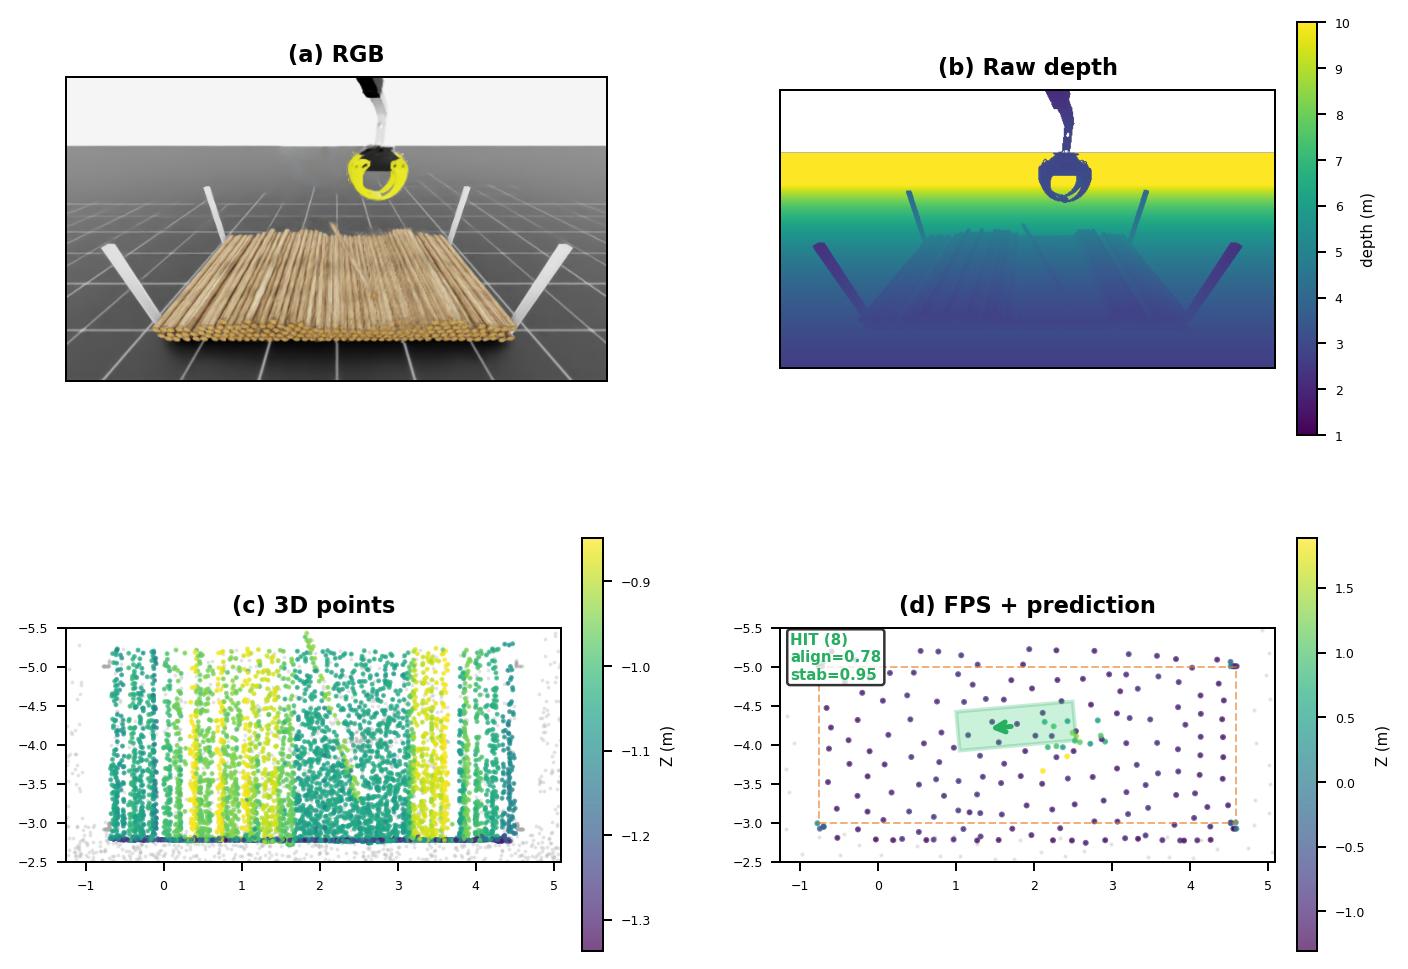
\includegraphics[width=\columnwidth]{episode_001_pipeline_quad_single.png}
\caption{Observation pipeline for a single grasp: RGB, raw depth, 3D back-projection in the crane base frame, and FPS-downsampled point cloud with the predicted grasp target and action-space bounds (dashed box).}
\label{fig:pcd_pipeline}
\end{figure}

As an ablation, we also evaluate policies that observe privileged per-object state: the top-$K$ log poses sorted by height (highest first), each represented as $(x,y,z,\psi)$ in the crane base frame.
Removed logs are excluded and remaining slots are padded with $-1$.
With $K\!=\!32$ this yields a compact $4K = 128$ dimensional vector.
This baseline isolates the effect of the perception gap: any performance difference between pose and point cloud policies is attributable to the observation representation rather than the learning algorithm.

\subsection{Actions}
\label{sec:actions}
The policy outputs a 5D vector $\tilde{a}_t \in \mathbb{R}^5$.
The first three components encode position and the remaining two encode grapple yaw.

Each position component is squashed via the hyperbolic tangent $\tanh$ and then linearly mapped to the per-environment workspace bounds to produce the base-frame target position $p^{\mathbf{b}}_i$:
\begin{equation}
    p^{\mathbf{b}}_i = \frac{(\tanh \tilde{a}_i + 1)}{2}(b_i^{\max} - b_i^{\min}) + b_i^{\min}, \quad i \in \{x,y,z\},
\end{equation}
where $b_i^{\min}, b_i^{\max}$ are the rack-aligned workspace limits for each axis.
These bounds are derived from the rack geometry with margins along each axis, yielding a workspace of approximately $2.0 \times 5.2 \times 1.0$\,m in the crane base frame.
Logs knocked outside the workspace are automatically removed and counted separately (Section~\ref{sec:outcome}). The heuristic expert (Section~\ref{sec:expert}) operates within the same bounds.

The remaining two components encode grapple yaw via the $\pi$-periodic pair $(\cos 2\psi, \sin 2\psi)$~\cite{morrison2018closing}. The yaw is recovered as $\psi = \tfrac{1}{2}\,\mathrm{atan2}(\tanh \tilde{a}_5,\;\tanh \tilde{a}_4) \in [-\tfrac{\pi}{2},\;\tfrac{\pi}{2}]$.

\subsection{Grasp Outcome}
\label{sec:outcome}
At the end of each grasp attempt, the outcome is evaluated by measuring three quantities:

\textbf{Logs grasped} ($g$): the number of active logs whose centers lie within a proximity radius of the closed grapple after lifting.

\textbf{Alignment} ($\alpha$): for each grasped log $i$, we compute per-log alignment $\alpha_i$ from the angle between the grapple $\hat{y}^{\mathbf{g}}$ axis and the log's length axis $\hat{y}^{\boldsymbol{\ell}}_i$ via their dot product (${\hat{y}^{\mathbf{g}}}^\top \hat{y}^{\boldsymbol{\ell}}_i = \cos\theta_{\alpha_i}$, where $\theta_{\alpha_i}$ is the misalignment angle).
Because a cylindrical log has no preferred length direction, the even exponent absorbs the sign; raising to the 8th power creates a sharp dropoff that penalizes moderate misalignment:
\begin{equation}
    \alpha_i = \big({\hat{y}^{\mathbf{g}}}^\top \hat{y}^{\boldsymbol{\ell}}_i\big)^{8}, \qquad \alpha = \frac{1}{g}\sum_{i=1}^{g} \alpha_i \;\in [0,1].
\end{equation}

\textbf{Stability} ($\varsigma$): the grapple's levelness after lifting, measured as ${\hat{z}^{\mathbf{g}}}^\top \hat{z}^{\mathbf{w}} = \cos\theta_\varsigma$, where $\theta_\varsigma$ is the tilt angle between the grapple's $z$-axis and the world vertical.
Clamping to zero excludes the degenerate case of an inverted grapple; raising to the 4th power ensures high scores only when the grapple is nearly level:
\begin{equation}
    \varsigma = \big(\max(0,\;{\hat{z}^{\mathbf{g}}}^\top \hat{z}^{\mathbf{w}})\big)^{4} \;\in [0,1].
\end{equation}
Logs identified as grasped are marked inactive and teleported out of the scene.
Logs that leave the workspace bounds during a grasp are removed and excluded from the grasp count $g$.
Figure~\ref{fig:grasp_geometry} visualizes the shaped score curves for alignment and stability.

\begin{figure}[t]
\centering

\includegraphics[width=\columnwidth]{outcomes.png}

\caption{Coordinate frames used to compute alignment ($\alpha$) and stability ($\varsigma$).}
\label{fig:grasp_geometry}
\end{figure}

\section{CONTROLLER AND ENVIRONMENT}

\begin{figure*}[t]
\centering
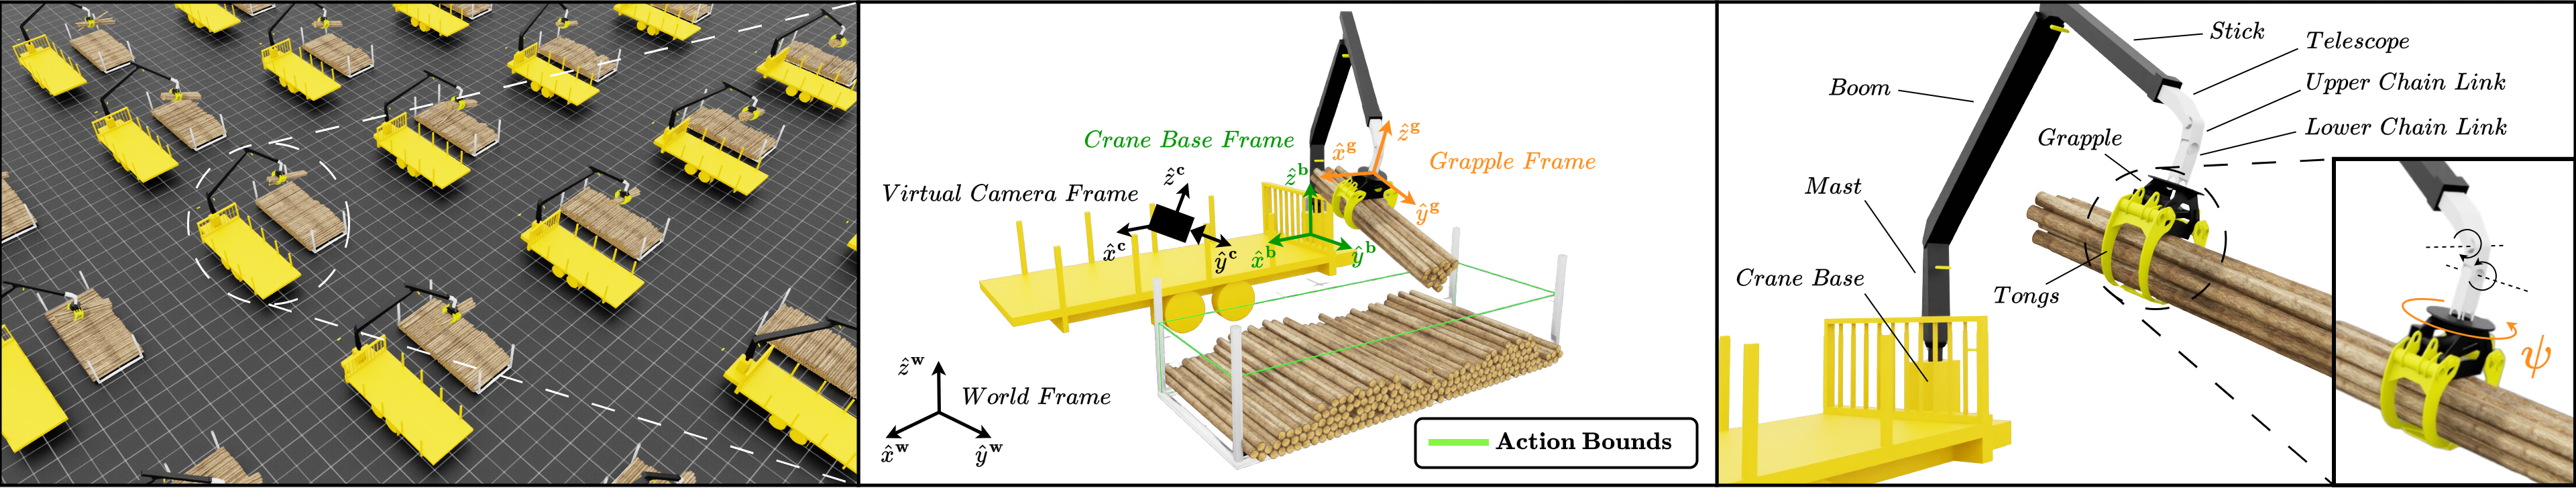
\includegraphics[width=\textwidth]{crane_env.png}
\caption{The grasp-and-remove crane environment. From left to right: parallelized training environments in Isaac Lab, each containing
a log loader crane above a rack of 200 logs in randomized configurations; a single environment showing the relevant coordinate frames
and the action-space bounding box; the crane articulation links, with the passive chain and grapple yaw joints highlighted.}
\label{fig:environment}
\end{figure*}

\subsection{Low-level Execution FSM}
All methods share the same fixed FSM controller, which runs at the control rate (60\,Hz, i.e., 120\,Hz physics with $2\times$ decimation) inside each environment step.
Given a grasp target $(x,y,z,\psi)$, produced by the heuristic (Section~\ref{sec:expert}) or a learned policy, the FSM executes a complete grasp cycle.

The crane arm has four actuated joints (base--mast, mast--boom, boom--stick, and stick--telescope) followed by a two-link passive chain that suspends the grapple from the telescope tip (Fig.~\ref{fig:environment}).
The two passive joints are unactuated revolute joints with low stiffness and damping, modeling the gravity-driven hanging behavior of a real forestry crane's grapple attachment.
Below the passive chain, a yaw joint actively rotates the grapple about the vertical axis, and two gripper joints control the grapple opening.

In this kinematic structure, the IK controller commands the top of the passive chain, but the grapple body hangs $0.415$\,m below it and swings like a pendulum during arm movements.
Consequently, all grasp targets are specified for the grapple body and then offset vertically to the IK target link.
The FSM uses a two-stage convergence check at each phase: it first waits for the IK target link to reach its target within $\epsilon_{\text{up}} = 0.10$\,m, then waits for the grapple body to settle within $\epsilon_{\text{g}} = 0.25$\,m.
Both must hold for $N_{\text{dwell}} = 30$ consecutive timesteps before the phase advances, ensuring that pendulum oscillations have damped before proceeding.

The FSM implements a five-phase grasp cycle: \texttt{HOVER} (move above target with $z_{\text{clear}} = 2.5$\,m clearance), \texttt{ALIGN} (rotate grapple to target yaw $\psi$), \texttt{DESCEND} (lower at 30\% speed to minimize disturbance), \texttt{CLOSE} (close grapple via discrete stepping), and \texttt{LIFT} (raise at 50\% speed, evaluate outcome per Section~\ref{sec:outcome}, remove grasped logs, open grapple, repeat).
A per-phase timeout (100 timesteps) forces advancement if convergence is not reached.

The arm is controlled using Isaac Lab's task-space Differential IK controller~\cite{mittal2025isaaclab} (damped least-squares, position command type), which computes joint position targets from the current end-effector pose and Jacobian.
The grapple yaw joint is controlled independently via a PD position controller.
The grapple opening is controlled using a PD velocity law with saturation and discrete stepping to avoid abrupt contact forces.

\subsection{Simulation Setup}
We implement the environment in Isaac Lab~\cite{mittal2025isaaclab} and run PhysX GPU dynamics for large-scale parallel simulation.
Log and contact parameters (Table~\ref{tab:sim_params}) are based on measurements of representative forestry logs and published friction coefficients for oak on oak~\cite{avallone2006marks}.
We use conservative contact modeling (simplified collision geometry on the grapple, tuned contact and rest offsets, and damping limits for logs) to reduce interpenetration and numerical jitter.

\begin{table}[t]
\centering
\caption{Simulation and controller parameters. Actuator gains are implicit PhysX joint-drive values; IK gains are the PD velocity controller used by the FSM.}
\label{tab:sim_params}
\scriptsize
\resizebox{\columnwidth}{!}{%
\begin{tabular}[t]{@{}lr@{}}
\toprule
\multicolumn{2}{l}{\textbf{\textit{Crane link masses}}} \\
\midrule
Mast / Boom / Stick & 290 / 172 / 70\,kg \\
Telescope / Passive chain & 25 / 9\,kg \\
\addlinespace[2pt]
\multicolumn{2}{l}{\textbf{\textit{Joint limits}}} \\
\midrule
Base--mast (revolute) & $\pm100^{\circ}$ \\
Mast--boom (revolute) & $-22^{\circ}$ to $+75^{\circ}$ \\
Boom--stick (revolute) & $-177^{\circ}$ to $+2^{\circ}$ \\
Stick--telescope (prismatic) & 0.13--1.80\,m \\
Telescope--grapple (revolute) & $\pm180^{\circ}$ \\
\addlinespace[2pt]
\multicolumn{2}{l}{\textbf{\textit{Log properties}}} \\
\midrule
Diameter / length & 0.11 / 2.45\,m \\
Mass & 15\,kg \\
$\mu_s$ / $\mu_k$ & 0.62 / 0.48 \\
Angular damping & 0.05 \\
Contact / rest offset & 0.02 / 0.0\,m \\
Max depenetration vel. & 3.0\,m/s \\
\bottomrule
\end{tabular}%
\hspace{8pt}%
\begin{tabular}[t]{@{}lr@{}}
\toprule
\multicolumn{2}{l}{\textbf{\textit{Simulation}}} \\
\midrule
Physics timestep ($\Delta t$) & $1/120$\,s \\
Control decimation & $2\times$ (60\,Hz) \\
\addlinespace[2pt]
\multicolumn{2}{l}{\textbf{\textit{Actuator gains}} ($k_p$ / $k_d$)} \\
\midrule
Main arm joints & $10^{6}$ / $10^{5}$ \\
Passive chain & 300 / 500 \\
Grapple yaw & $5\!\times\!10^{4}$ / $2\!\times\!10^{4}$ \\
Grapple tongs & 0 / 500 \\
\addlinespace[2pt]
\multicolumn{2}{l}{\textbf{\textit{IK PD gains}} ($k_p$ / $k_d$)} \\
\midrule
Arm joints & 4.0 / 1.2 \\
Grapple tongs & 12.0 / 1.0 \\
\addlinespace[2pt]
\multicolumn{2}{l}{\textbf{\textit{FSM parameters}}} \\
\midrule
Hover clearance & 2.5\,m \\
Pos.\ tol.\ (passive / grapple) & 0.10 / 0.25\,m \\
Dwell count & 30 steps \\
Phase timeout & 100 steps \\
\bottomrule
\end{tabular}%
}
\end{table}

\section{LEARNING}

\subsection{Heuristic Expert}
\label{sec:expert}
We implement a hand-tuned heuristic expert that serves as the demonstration source for BC and as a privileged-state comparison.
The heuristic has access to privileged information (the position and orientation of every active log from the physics engine) and uses a deterministic top-of-pile targeting strategy:

At each pick cycle, the expert selects the topmost active log (highest $z$-coordinate), transforms its center into the crane base frame as the $(x,y,z)$ target, and aligns the grapple yaw $\psi$ with the log's length axis (choosing the orientation requiring minimal joint rotation).
The target $z$ is set $0.6$\,m above the topmost log's center, hand-tuned to balance throughput: lower values choke the grapple with too many logs, higher values reduce the number captured per grasp.
This strategy is effective because the highest log is typically the most accessible, but does not adapt in the endgame when few scattered logs remain. Despite this, the expert achieves strong performance across all metrics (Table~\ref{tab:results}).

\subsection{Behavior Cloning}
\label{sec:bc}
We use BC to train a policy from expert demonstrations.
We collect demonstration pairs $(o_t, a_t^*)$ from successful expert grasps only (failed grasps are discarded), where $o_t$ is the point cloud observation and $a_t^*$ is the expert action in the pre-squashing space (positions via $\tanh^{-1}$, yaw via $\cos 2\psi, \sin 2\psi$ as described in Section~\ref{sec:actions}).

The policy uses a PointNet encoder~\cite{qi2017pointnet}.
A shared per-point MLP $h: \mathbb{R}^3 \to \mathbb{R}^{256}$ (layers $3 \!\to\! 64 \!\to\! 128 \!\to\! 256$ with batch normalization and ELU activations) maps each point independently; a symmetric max-pool aggregates the per-point features, and a post-pooling fully connected layer $f_{\mathrm{fc}}$ ($256 \!\to\! 256$, BN, ELU) yields the global latent vector:
\begin{equation}
    \mathbf{z} = f_{\mathrm{fc}}\!\Big(\max_{i=1,\ldots,N_p} h\!\big(o_{t,i}\big)\Big) \;\in \mathbb{R}^{256},
\end{equation}
where $o_{t,i} \in \mathbb{R}^3$ is the $i$-th point in the observation.
An actor MLP $\mu_\theta: \mathbb{R}^{256} \to \mathbb{R}^{5}$ (layers $256 \!\to\! 128 \!\to\! 64 \!\to\! 5$) maps the latent to the action $\tilde{a}_t = \mu_\theta(\mathbf{z})$.
For the privileged-pose ablation, we replace the PointNet encoder with a three-layer MLP ($128 \!\to\! 256 \!\to\! 128 \!\to\! 64$) with ELU activations.

We apply dropout (rate 0.2) after the encoder.
The BC objective minimizes the mean-squared error between the predicted and expert actions over a dataset $\mathcal{D}$ of successful grasps:
\begin{equation}
    \mathcal{L}_{\text{BC}} = \frac{1}{|\mathcal{D}|}\sum_{(o,a^*)\in\mathcal{D}} \left\| \mu_\theta(\mathbf{z}) - a^* \right\|^2,
\end{equation}
where $\mathbf{z}$ is the encoder output for observation $o$.
We optimize with AdamW~\cite{loshchilov2019adamw} (learning rate $10^{-4}$, weight decay $10^{-4}$) with the learning rate halved whenever validation loss plateaus for 10 epochs.
The training dataset was collected from 1{,}000 episodes and contains $\sim$20{,}700 successful-grasp samples ($\sim$85/15 train/validation split). The raw PC model is selected by minimum validation loss (0.101 MSE, epoch 190) with early stopping (patience 30 epochs).

\subsection{Reinforcement Learning}
\label{sec:rl}
We train policies with PPO~\cite{schulman2017ppo} using the RSL-RL library~\cite{schwarke2025rslrl}.
PPO optimizes a stochastic Gaussian policy with parameters $\theta$:
\begin{equation}
    \pi_\theta(a \mid s) = \mathcal{N}\!\big(\mu_\theta(s),\;\mathrm{diag}(\bm{\sigma}^2)\big),
\end{equation}
where $\mu_\theta$ outputs the mean action and $\bm{\sigma} \in \mathbb{R}^{|\mathcal{A}|}$ is a learnable standard deviation vector initialized to $\sigma_0 \mathbf{1}$.
A separate critic $V_\phi(s)$ estimates the state-value function; advantages are computed via Generalized Advantage Estimation (GAE)~\cite{schulman2017ppo}.

The actor uses the same PointNet encoder and actor MLP as the BC policy; the critic uses an independent PointNet encoder with its own MLP head.
For the privileged-pose ablation, both actor and critic are separate MLPs with hidden dimensions $[256, 128, 64]$ and ELU activations.
Key hyperparameters: $\sigma_0 = 1.0$, clipping ratio $\epsilon=0.2$, entropy coefficient $0.01$, learning rate $3\times10^{-4}$ with adaptive KL-based scheduling (target KL $0.01$), GAE with $\lambda=0.95$, discount factor $\gamma = 0.99$, five learning epochs with four mini-batches per epoch, and gradient clipping at norm $1.0$.
Each iteration collects $N_{\text{env}} \times 4$ grasp cycles (one step per cycle) across all parallel environments and performs one PPO update; total grasp experience after $k$ iterations is therefore $4 k N_{\text{env}}$.
The outcome components $(g,\alpha,\varsigma)$ from Section~\ref{sec:outcome} define the scalar reward:
\label{eq:reward}
\begin{equation}
r = g \cdot \alpha \cdot \varsigma,
\end{equation}
for successful grasps ($g > 0$), and $r = -1$ for failed grasps.
The reward is thus the product of throughput, alignment, and stability; a high reward requires many logs grasped with good alignment and a level grapple.
The reward is entirely per-grasp.
Global pile-clearing ability must emerge from the policy's targeting strategy rather than from explicit reward incentives.
We also train two reward variants to test sensitivity to reward formulation.
First, a \emph{throughput-only} reward $r = g$ removes the alignment and stability terms, testing whether quality constraints encourage a conservative strategy that maximizes per-grasp return at the expense of pile progress.
Second, a \emph{normalized} reward $r = c \cdot (g/n_\ell) \cdot \alpha \cdot \varsigma$, where $n_\ell = \min(\max(1, n_{\ell,\mathrm{raw}}),\, 15)$ is the number of available logs beneath the grapple target (capped near grapple capacity) and $c = 10$ is a scale constant, equalizes early and late grasps: when the pile is dense $n_\ell$ is large and when it is sparse $n_\ell$ is small, so a policy that takes what is available receives comparable reward regardless of pile state.





\subsection{BC-Initialized RL Fine-Tuning}
\label{sec:bcrl}






To combine BC's full-trajectory coverage with RL's ability to optimize per-grasp metrics, we initialize a PPO agent from the trained BC policy and fine-tune with on-policy experience~\cite{rajeswaran2018learning, nair2018overcoming}.

The BC actor weights (PointNet encoder and actor MLP) are loaded into the PPO actor (Fig.~\ref{fig:bcrl_pipeline}); the critic is initialized randomly and the optimizer starts fresh.
We use an asymmetric actor-critic~\cite{pinto2018asymmetric}: the actor observes the raw point cloud (same as BC), while the critic is a trainable MLP that receives the privileged top-$K$ log poses.
This asymmetry allows the critic to learn a more accurate value function from compact state information, while the actor retains the vision-based input it will use at deployment.

We freeze the BC-trained PointNet encoder during RL fine-tuning: the asymmetric critic cannot propagate gradients through the encoder, so an unfrozen encoder drifts without constraint and fine-tuning the full network causes training collapse.

All other PPO hyperparameters remain identical to the from-scratch RL configuration (Section~\ref{sec:rl}); the only changes are the frozen encoder and a reduced initial policy noise $\sigma_0 = 0.05$ (vs.\ $1.0$ for from-scratch RL), which limits exploration to small perturbations around the BC mean; higher noise causes gradual degradation ($\sigma_0 = 0.1$) or rapid collapse ($\sigma_0 = 0.3$).


\begin{figure*}[t]
\centering
\resizebox{0.92\textwidth}{!}{%
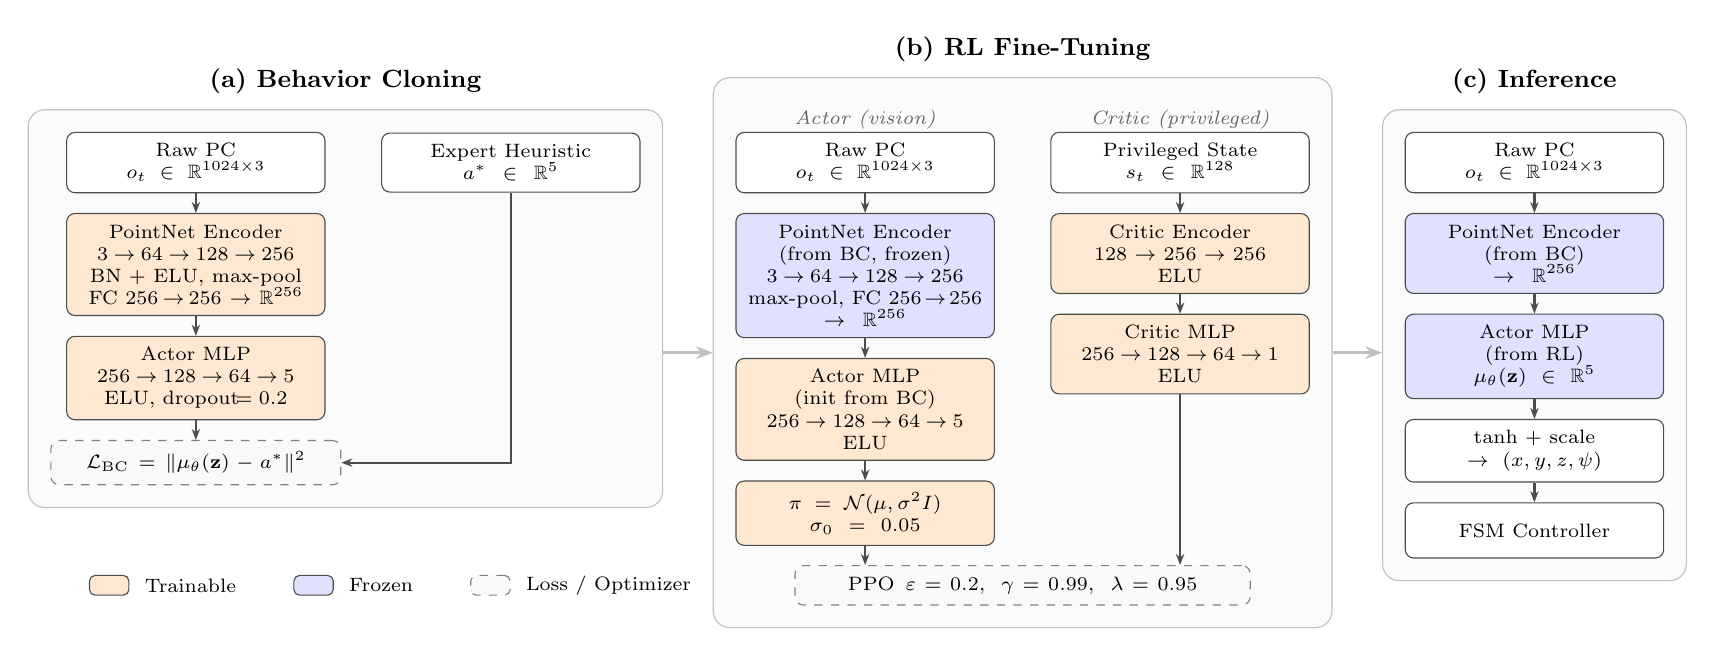
\begin{tikzpicture}[
  block/.style={rectangle, rounded corners=3pt, draw=black!70,
    text width=3.0cm, minimum height=0.7cm, align=center,
    font=\scriptsize, inner sep=4pt},
  frozen/.style={block, fill=blue!12},
  trainable/.style={block, fill=orange!18},
  io/.style={block, fill=white},
  lossnode/.style={rectangle, rounded corners=3pt, draw=black!50, dashed,
    text width=3.4cm, align=center, font=\scriptsize, inner sep=4pt, fill=gray!5},
  wideloss/.style={lossnode, text width=5.5cm},
  arr/.style={-{Stealth[length=4pt]}, thick, black!70},
  panelbg/.style={rectangle, rounded corners=6pt, draw=gray!50,
    fill=gray!3, inner sep=8pt},
  ptitle/.style={font=\small\bfseries},
  collabel/.style={font=\scriptsize\itshape, text=black!60},
]
% ====== PANEL (a): BEHAVIOR CLONING ======
\node[io] (a_pcd) at (0, 0)
  {Raw PC\\$o_t \in \mathbb{R}^{1024\times3}$};
\node[io] (a_expert) at (4, 0)
  {Expert Heuristic\\$a^{*} \in \mathbb{R}^{5}$};
\node[trainable, below=0.25cm of a_pcd] (a_enc)
  {PointNet Encoder\\$3\!\to\!64\!\to\!128\!\to\!256$\\BN + ELU, max-pool\\FC $256\!\to\!256 \to\mathbb{R}^{256}$};
\node[trainable, below=0.25cm of a_enc] (a_mlp)
  {Actor MLP\\$256\!\to\!128\!\to\!64\!\to\!5$\\ELU, dropout$\!=\!0.2$};
\node[lossnode, below=0.25cm of a_mlp] (a_loss)
  {$\mathcal{L}_{\text{BC}} = \lVert\mu_\theta(\mathbf{z}) - a^{*}\rVert^{2}$};
\draw[arr] (a_pcd) -- (a_enc);
\draw[arr] (a_enc) -- (a_mlp);
\draw[arr] (a_mlp) -- (a_loss);
\draw[arr] (a_expert.south) |- (a_loss.east);
%
% ====== PANEL (b): RL FINE-TUNING ======
\node[collabel] (b_alabel) at (8.5, 0.55) {Actor (vision)};
\node[collabel] (b_clabel) at (12.5, 0.55) {Critic (privileged)};
% Actor column
\node[io] (b_pcd) at (8.5, 0) {Raw PC\\$o_t \in \mathbb{R}^{1024\times3}$};
\node[frozen, below=0.25cm of b_pcd] (b_enc)
  {PointNet Encoder\\(from BC, frozen)\\$3\!\to\!64\!\to\!128\!\to\!256$\\max-pool, FC $256\!\to\!256$\\$\to\mathbb{R}^{256}$};
\node[trainable, below=0.25cm of b_enc] (b_actor)
  {Actor MLP\\(init from BC)\\$256\!\to\!128\!\to\!64\!\to\!5$\\ELU};
\node[trainable, below=0.25cm of b_actor] (b_policy)
  {$\pi = \mathcal{N}(\mu, \sigma^{2} I)$\\$\sigma_0 = 0.05$};
% Critic column
\node[io] (b_state) at (12.5, 0)
  {Privileged State\\$s_t \in \mathbb{R}^{128}$};
\node[trainable, below=0.25cm of b_state] (b_cenc)
  {Critic Encoder\\$128\!\to\!256\!\to\!256$\\ELU};
\node[trainable, below=0.25cm of b_cenc] (b_cmlp)
  {Critic MLP\\$256\!\to\!128\!\to\!64\!\to\!1$\\ELU};
% PPO node spanning both columns (anchored below deepest column, centered)
\path (b_policy.south) ++(0,-0.5) coordinate (ppo_y);
\path (b_pcd.center) -- (b_state.center) coordinate[midway] (ppo_x);
\node[wideloss] (b_ppo) at (ppo_y -| ppo_x)
  {PPO\enspace $\varepsilon\!=\!0.2,\;\gamma\!=\!0.99,\;\lambda\!=\!0.95$};
\draw[arr] (b_pcd) -- (b_enc);
\draw[arr] (b_enc) -- (b_actor);
\draw[arr] (b_actor) -- (b_policy);
\draw[arr] (b_state) -- (b_cenc);
\draw[arr] (b_cenc) -- (b_cmlp);
\draw[arr] (b_policy.south) -- (b_policy |- b_ppo.north);
\draw[arr] (b_cmlp.south) -- (b_cmlp |- b_ppo.north);
%
% ====== PANEL (c): INFERENCE ======
\node[io] (c_pcd) at (17, 0) {Raw PC\\$o_t \in \mathbb{R}^{1024\times3}$};
\node[frozen, below=0.25cm of c_pcd] (c_enc)
  {PointNet Encoder\\(from BC)\\$\to\mathbb{R}^{256}$};
\node[frozen, below=0.25cm of c_enc] (c_actor)
  {Actor MLP\\(from RL)\\$\mu_\theta(\mathbf{z}) \in \mathbb{R}^{5}$};
\node[io, below=0.25cm of c_actor] (c_scale)
  {tanh + scale\\$\to(x,y,z,\psi)$};
\node[io, below=0.25cm of c_scale] (c_fsm) {FSM Controller};
\draw[arr] (c_pcd) -- (c_enc);
\draw[arr] (c_enc) -- (c_actor);
\draw[arr] (c_actor) -- (c_scale);
\draw[arr] (c_scale) -- (c_fsm);
%
% ====== PANEL BACKGROUNDS (consolidated, natural height per panel) ======
\begin{scope}[on background layer]
  \node[panelbg, fit=(a_pcd)(a_expert)(a_enc)(a_mlp)(a_loss)] (bg_a) {};
  \node[panelbg, fit=(b_alabel)(b_clabel)(b_pcd)(b_enc)(b_actor)(b_policy)(b_state)(b_cenc)(b_cmlp)(b_ppo)] (bg_b) {};
  \node[panelbg, fit=(c_pcd)(c_enc)(c_actor)(c_scale)(c_fsm)] (bg_c) {};
\end{scope}
\node[ptitle, above=2pt of bg_a.north] {(a) Behavior Cloning};
\node[ptitle, above=2pt of bg_b.north] {(b) RL Fine-Tuning};
\node[ptitle, above=2pt of bg_c.north] {(c) Inference};
%
% ====== STAGE ARROWS (level, pinned to panel b midpoint) ======
\draw[-{Stealth[length=6pt]}, very thick, gray!50]
  (bg_a.east |- bg_b.west) -- (bg_b.west);
\draw[-{Stealth[length=6pt]}, very thick, gray!50]
  (bg_b.east) -- (bg_c.west |- bg_b.east);
%
% ====== LEGEND ======
\coordinate (leg_start) at ($(bg_a.center |- b_ppo) + (-3.0, 0)$);
\node[rectangle, rounded corners=2pt, draw=black!70, fill=orange!18,
  minimum width=0.5cm, minimum height=0.25cm] (leg_t) at (leg_start) {};
\node[font=\scriptsize, right=2pt of leg_t] (leg_tl) {Trainable};
\node[rectangle, rounded corners=2pt, draw=black!70, fill=blue!12,
  minimum width=0.5cm, minimum height=0.25cm, right=0.6cm of leg_tl] (leg_f) {};
\node[font=\scriptsize, right=2pt of leg_f] (leg_fl) {Frozen};
\node[rectangle, rounded corners=2pt, draw=black!50, dashed, fill=gray!5,
  minimum width=0.5cm, minimum height=0.25cm, right=0.6cm of leg_fl] (leg_l) {};
\node[font=\scriptsize, right=2pt of leg_l] {Loss / Optimizer};
\end{tikzpicture}%
}% end resizebox
\caption{The BC$\to$RL pipeline. (a)~The PointNet encoder and actor MLP are trained end-to-end on expert demonstrations with MSE loss. (b)~The encoder is frozen and the actor MLP is fine-tuned with PPO alongside a state-based asymmetric critic. (c)~At inference the critic is discarded; the encoder and actor run deterministically.}
\label{fig:bcrl_pipeline}
\end{figure*}
\begin{figure}[t]
\centering
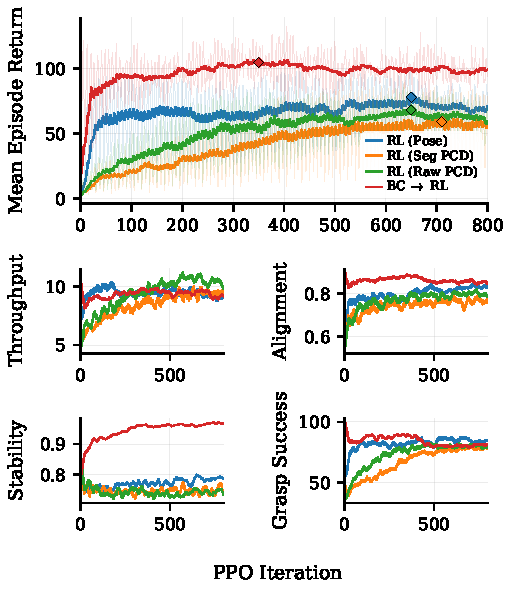
\includegraphics[width=\columnwidth]{reward_curves.pdf}
\caption{PPO training curves. Mean episode return vs.\ PPO iteration (bold: 20-iteration rolling average; shading: raw). Diamond markers indicate the evaluation checkpoint. Bottom panels show per-grasp reward components and success rate.}
\label{fig:reward_curves}
\end{figure}
\begin{figure}[tb]
\centering
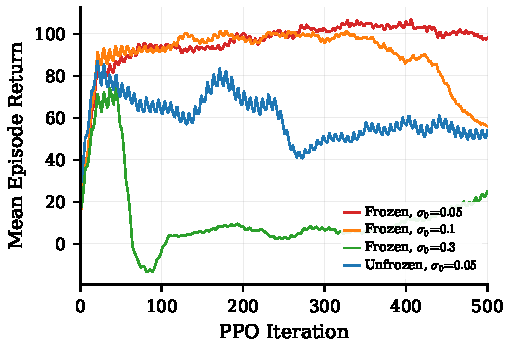
\includegraphics[width=\columnwidth]{bcrl_ablation_minimal.pdf}
\caption{BC+RL training sensitivity. Mean episode return vs.\ PPO iteration for four configurations varying encoder freezing and initial policy noise $\sigma_0$.}
\label{fig:bcrl_ablation}
\end{figure}
\section{EXPERIMENTS}
\subsection{Setup}
All experiments use the same crane model, rack geometry, and FSM controller, and run on a single NVIDIA RTX 4070 Laptop GPU (8\,GB VRAM).
Training uses 32 parallel environments for pose-based policies and 20 for point cloud policies (Fig.~\ref{fig:environment}).
Piles contain 200 cylindrical logs spawned in layered grid patterns with randomized grid dimensions, spacing ($\pm 5$--$15$\%), layer offsets, and per-log placement jitter.
The log count is fixed at 200 for the main comparisons so that clearing metrics are directly comparable between methods; the pile variation rows (Table~\ref{tab:results}) additionally randomize log count ($20$--$200$) to test generalization across different pile sizes and initial conditions.

Each episode runs for $H=30$ grasp attempts (Section~\ref{sec:formulation}). We evaluate over 100 episodes on identical random seeds across 20 parallel environments; all metrics are per-episode mean $\pm$ standard deviation.

To evaluate robustness to sensor noise, we add isotropic Gaussian noise $\mathcal{N}(0, \sigma_{\mathrm{obs}}^2 I)$ to each point in the cloud at evaluation time.
The ZED~X achieves depth errors below $0.8\%$ at $2$\,m\footnote{\href{https://cdn.sanity.io/files/s18ewfw4/staging/ec78a504b36ab95d6620ac720ffa5feaa2e8948b.pdf/ZED\%20X\%20Datasheet\%20v1.2.pdf}{ZED~X Datasheet v1.2}}, so $\sigma_{\mathrm{obs}} = 0.05$\,m represents a conservative upper bound on real sensor noise at typical operating distances.
We sweep $\sigma_{\mathrm{obs}} \in \{0.05, 0.1, 0.2\}$\,m to stress-test robustness up to severe corruption.
The policy receives only $1{,}024$ FPS-downsampled points that include background geometry (crane, rack, floor) alongside the pile, making this a particularly stringent test of robustness.


\subsection{Metrics}
\label{sec:metrics}
We report metrics derived from the outcome tuple $(g, \alpha, \varsigma)$ (Section~\ref{sec:outcome}), all as per-episode mean $\pm$ std: \emph{throughput} (mean logs per successful grasp), \emph{alignment} (grasp-count-weighted mean $\alpha$), \emph{stability} (mean $\varsigma$ over successful grasps), \emph{grasp success rate} (fraction with $g>0$), \emph{clearing rate} (fraction of logs intentionally removed), and \emph{knocked-off percentage} (fraction knocked outside bounds). We also report $c_{95}$, the number of grasp cycles needed to clear 95\% of the pile. We use 95\% rather than 100\% because the final logs may rest flat on the ground or settle in awkward orientations, requiring disproportionately more attempts than stacked logs.



\begin{table*}[!t]
\centering
\caption{Evaluation metrics (mean $\pm$ std, 100 episodes). All piles use randomized placement. Upper rows: 200-log piles. Lower sections: reward ablation, pile size variation (20--200 logs), and point cloud noise robustness. The heuristic uses privileged pose state. Best per column among raw point-cloud methods in \textbf{bold}.}
\label{tab:results}
\scriptsize
\setlength{\tabcolsep}{3pt}
\setlength{\aboverulesep}{0.2ex}
\setlength{\belowrulesep}{0.4ex}
\renewcommand{\arraystretch}{0.85}
\begin{tabular*}{\textwidth}{@{\extracolsep{\fill}}llccccccc@{}}
\toprule
Method & Obs. & $g$ & $\alpha$ & $\varsigma$ & Grasp succ.\,(\%) & Clear rate\,(\%) & Knocked off\,(\%) & $c_{95}$ \\
\midrule
Heuristic & Pose & $9.94 \pm 1.17$ & $0.918 \pm 0.031$ & $0.797 \pm 0.018$ & $88.7 \pm 7.8$ & $99.0 \pm 1.2$ & $1.0 \pm 1.1$ & $18.8 \pm 2.8$ \\
\addlinespace
RL & Pose (128D) & $8.51 \pm 1.27$ & $0.874 \pm 0.054$ & $0.958 \pm 0.014$ & $58.7 \pm 10.4$ & $73.3 \pm 7.2$ & $0.6 \pm 0.6$ & N/A \\
RL & Seg.\ PC   & $7.65 \pm 0.98$ & $0.772 \pm 0.065$ & $0.737 \pm 0.044$ & $47.4 \pm 6.8$ & $53.4 \pm 3.1$ & $0.5 \pm 0.5$ & N/A \\
RL & Raw PC     & $6.78 \pm 1.01$ & $0.758 \pm 0.072$ & $0.815 \pm 0.039$ & $53.3 \pm 8.7$ & $53.0 \pm 3.9$ & $\mathbf{0.6 \pm 0.6}$ & N/A \\
\addlinespace
BC & Seg.\ PC   & $9.64 \pm 1.05$ & $0.907 \pm 0.028$ & $0.816 \pm 0.020$ & $70.3 \pm 10.6$ & $96.5 \pm 4.7$ & $0.9 \pm 1.0$ & $21.7 \pm 4.6$ \\
BC & Raw PC     & $\mathbf{9.32 \pm 1.12}$ & $0.904 \pm 0.037$ & $0.824 \pm 0.025$ & $84.5 \pm 9.8$ & $\mathbf{98.5 \pm 5.1}$ & $0.7 \pm 0.7$ & $\mathbf{20.6 \pm 3.0}$ \\
\addlinespace
BC$\to$RL & Raw PC & $8.65 \pm 0.97$ & $\mathbf{0.906 \pm 0.027}$ & $\mathbf{0.947 \pm 0.016}$ & $\mathbf{86.3 \pm 8.5}$ & $98.2 \pm 1.5$ & $1.2 \pm 0.8$ & $21.9 \pm 3.2$ \\
\midrule
\multicolumn{9}{l}{\textit{Reward ablation}} \\
\midrule
RL ($r{=}g$) & Raw PC & $6.93 \pm 1.10$ & $0.747 \pm 0.087$ & $0.716 \pm 0.059$ & $53.3 \pm 8.8$ & $54.2 \pm 4.3$ & $1.6 \pm 1.6$ & N/A \\
RL (norm.)   & Raw PC & $6.72 \pm 0.92$ & $0.750 \pm 0.063$ & $0.759 \pm 0.065$ & $48.8 \pm 7.9$ & $48.3 \pm 4.0$ & $0.3 \pm 0.5$ & N/A \\
\midrule
\multicolumn{9}{l}{\textit{Pile size variation (20--200 logs)}} \\
\midrule
Heuristic & Pose   & $8.28 \pm 1.96$ & $0.889 \pm 0.074$ & $0.789 \pm 0.024$ & $86.3 \pm 11.6$ & $98.2 \pm 4.9$ & $1.3 \pm 1.6$ & $13.6 \pm 4.9$ \\
\addlinespace
BC        & Raw PC & $7.55 \pm 2.02$ & $0.860 \pm 0.093$ & $0.820 \pm 0.029$ & $72.8 \pm 17.7$ & $98.4 \pm 2.5$ & $1.2 \pm 1.5$ & $15.8 \pm 4.9$ \\
BC$\to$RL & Raw PC & $6.97 \pm 1.63$ & $0.861 \pm 0.081$ & $0.922 \pm 0.037$ & $76.0 \pm 14.9$ & $98.5 \pm 1.5$ & $1.3 \pm 1.4$ & $16.4 \pm 4.9$ \\
\midrule
\multicolumn{9}{l}{\textit{Point cloud noise (isotropic Gaussian, $\sigma_{\mathrm{obs}}$ in m)}} \\
\midrule
BC        & Raw PC ($\sigma_{\mathrm{obs}}{=}0.05$) & $9.08 \pm 0.89$ & $0.897 \pm 0.029$ & $0.831 \pm 0.019$ & $83.9 \pm 10.0$ & $99.0 \pm 0.9$ & $0.7 \pm 0.7$ & $20.8 \pm 2.4$ \\
BC        & Raw PC ($\sigma_{\mathrm{obs}}{=}0.1$)  & $6.80 \pm 0.67$ & $0.858 \pm 0.040$ & $0.871 \pm 0.016$ & $81.7 \pm 6.6$ & $83.2 \pm 8.8$ & $1.0 \pm 0.8$ & $29.9 \pm 0.7$ \\
BC        & Raw PC ($\sigma_{\mathrm{obs}}{=}0.2$)  & $4.32 \pm 0.82$ & $0.839 \pm 0.065$ & $0.951 \pm 0.024$ & $49.3 \pm 7.5$ & $31.3 \pm 3.7$ & $0.5 \pm 0.5$ & N/A \\
\addlinespace
BC$\to$RL & Raw PC ($\sigma_{\mathrm{obs}}{=}0.05$) & $8.92 \pm 0.99$ & $0.913 \pm 0.027$ & $0.967 \pm 0.011$ & $89.4 \pm 8.2$ & $98.7 \pm 0.9$ & $1.2 \pm 0.8$ & $21.1 \pm 2.5$ \\
BC$\to$RL & Raw PC ($\sigma_{\mathrm{obs}}{=}0.1$)  & $7.73 \pm 0.77$ & $0.875 \pm 0.034$ & $0.954 \pm 0.015$ & $83.3 \pm 6.6$ & $93.9 \pm 5.9$ & $1.3 \pm 0.8$ & $27.5 \pm 3.1$ \\
BC$\to$RL & Raw PC ($\sigma_{\mathrm{obs}}{=}0.2$)  & $5.30 \pm 0.78$ & $0.734 \pm 0.072$ & $0.833 \pm 0.042$ & $66.6 \pm 7.4$ & $52.6 \pm 7.5$ & $1.7 \pm 1.0$ & N/A \\
\bottomrule
\end{tabular*}
\end{table*}
\section{RESULTS}
\label{sec:results}

Table~\ref{tab:results} summarizes the evaluation metrics.
All four methods share the same controller, pile configuration, and evaluation protocol; the only differences are the targeting policy and its observation.
From-scratch RL uses a symmetric actor-critic in which both actor and critic process observations through independent encoders (PointNet for PC variants, MLPs for the pose ablation).
BC+RL uses an asymmetric actor-critic~\cite{pinto2018asymmetric} in which the actor retains the frozen BC-trained PointNet encoder while the critic is a trainable MLP that receives the privileged state vector (Section~\ref{sec:bcrl}).


From-scratch RL achieves competitive per-grasp reward during training (Fig.~\ref{fig:reward_curves}; shading reflects episode variability within a run): RL~(Pose) converges to a mean episode reward of $\sim$95--97 within 80 iterations, while RL~(PC) reaches $\sim$85--90 after several hundred iterations.
However, high training reward does not translate to pile-clearing performance.
The privileged-pose variant clears more than either PC variant but still falls far short of the heuristic (Table~\ref{tab:results}), indicating that the primary bottleneck is exploration rather than perception alone.
The reward ablation (Table~\ref{tab:results}, lower RL rows) tests whether the clearing plateau is caused by the reward formulation; both variants plateau near ${\sim}50\%$ clearing, matching the combined-reward baseline and suggesting the clearing gap is independent of reward formulation.

BC achieves 98.5\% clearing using only raw point clouds, comparable to the privileged-state heuristic (99.0\%).
Conditional per-grasp metrics closely match the heuristic, with the largest gap in grasp success rate (84.5\% vs.\ 88.7\%).
Raw PC yields a notably higher grasp success rate than segmented PC (84.5\% vs.\ 70.3\%) with comparable clearing.

BC+RL fine-tuning improves grasp stability from $\varsigma = 0.824$ (BC) to $0.947$, also surpassing the privileged-state heuristic ($0.797$), while preserving full-trajectory clearing.
Alignment remains comparable and throughput is slightly lower ($8.65$ vs.\ $9.32$).
Figure~\ref{fig:bcrl_ablation} shows that both the frozen encoder and conservative noise are necessary: higher noise or an unfrozen encoder each cause training collapse.

The lower rows of Table~\ref{tab:results} report all metrics under increasing point cloud noise.
BC$\to$RL retains 93.9\% clearing at $\sigma_{\mathrm{obs}} = 0.1$\,m, whereas BC drops to 83.2\%; both degrade sharply at $\sigma_{\mathrm{obs}} = 0.2$\,m.
Despite aggressive FPS downsampling to just $1{,}024$ points, both learned policies are noise-tolerant; RL fine-tuning further improves this robustness beyond BC alone.

\section{DISCUSSION}
The near-identical clearing of BC and BC+RL confirms that RL fine-tuning preserves the expert's clearing ability while improving grasp stability. Under the combined reward ($g \cdot \alpha \cdot \varsigma$), RL achieves high per-grasp scores during training yet clears far less than the expert at evaluation. Because the reward scores each grasp independently (Section~\ref{sec:rl}), a policy can achieve high return without developing a targeting strategy that completes the full sequence. Privileged pose access improves clearing relative to point clouds but does not close the gap to the heuristic, and neither reward ablation alters this conclusion.

BC initialization provides a policy that already covers the full clearing sequence from dense stacks to sparse endgames~\cite{rajeswaran2018learning}. RL fine-tuning improves per-grasp execution without rediscovering the global targeting strategy. The encoder must remain frozen: the asymmetric critic provides no gradient to the visual pathway (Section~\ref{sec:bcrl}), and low noise ($\sigma_0 = 0.05$) prevents overwriting the learned policy.

Operating directly on depth-derived point clouds simplifies the perception pipeline and reduces potential failure modes. Both learned policies perform well at $\sigma_{\mathrm{obs}} = 0.1$\,m (Table~\ref{tab:results}), which exceeds expected real sensor noise at typical operating distances, suggesting robustness to real stereo-depth observations. Under pile variation, both learned policies maintain strong clearing; throughput and grasp success decrease modestly as irregular configurations present fewer easy multi-log grasps, with the heuristic dropping less due to its privileged state access.

The 15\% stability improvement from RL fine-tuning is practically significant: in real forestry operations, an unstable grasp causes load swing, increasing cycle time, hindering deposition, and raising operator risk. Achieving this improvement without sacrificing clearing rate is the key benefit of the BC$\to$RL approach.

Our design has limitations: removed logs are teleported (omitting deposition), and all experiments are in simulation. Architectures exploiting local geometry, such as point transformers, may improve endgame targeting. Despite these simplifications, the environment captures the essential challenges of sequential multi-log grasping from dense piles.

\section{CONCLUSION}
We presented a grasp-and-remove formulation for log-pile clearing at scale and a BC$\to$RL pipeline for learning stable grasps from raw point clouds. We further compared four targeting methods on a shared controller.
From-scratch RL falls well short of full clearing regardless of observation type or reward formulation; BC from raw point clouds matches the privileged-state heuristic; BC$\to$RL fine-tuning improves grasp stability by 15\% over BC while maintaining near-complete clearing.
Future work will explore sim-to-real transfer, richer point cloud architectures, and curriculum learning approaches to the exploration challenge.

\addtolength{\textheight}{-12cm}  % Balance column lengths on last page (adjust as needed)

\section*{ACKNOWLEDGMENT}
[Redacted for anonymity]

\bibliographystyle{IEEEtran}
\bibliography{references}

\end{document}
